\documentclass[11pt]{beamer}
\usepackage[utf8]{inputenc}
\usepackage[T1]{fontenc}
\usepackage{lmodern}
\usepackage[french]{babel}
\usetheme{Antibes}
\usepackage{subfig}
\usepackage{algorithm}
\usepackage{algorithmic}

\renewcommand{\algorithmicrequire}{\textbf{Entrée(s) :}}
\renewcommand{\algorithmicreturn}{\textbf{retourner}}
\renewcommand{\algorithmicensure}{\textbf{Initialisation ;}}
\renewcommand{\algorithmicwhile}{\textbf{Tant que}}
\renewcommand{\algorithmicdo}{\textbf{Initialisation}}
\renewcommand{\algorithmicendwhile}{\textbf{fin du Tant que ;}}
\renewcommand{\algorithmicend}{\textbf{fin}}
\renewcommand{\algorithmicif}{\textbf{si}}
\renewcommand{\algorithmicendif}{\textbf{fin du si}}
\renewcommand{\algorithmicelse}{\textbf{sinon}}
\renewcommand{\algorithmicelsif}{\textbf{fin du sinon}}
\renewcommand{\algorithmicthen}{\textbf{alors}}
\renewcommand{\algorithmicthen}{\textbf{Étape E}}
\renewcommand{\algorithmicthen}{\textbf{Étape M}}
\renewcommand{\algorithmicfor}{\textbf{pour}}
\renewcommand{\algorithmicforall}{\textbf{pour tout}}
\renewcommand{\algorithmicto}{\textbf{à}}
\renewcommand{\algorithmicendfor}{\textbf{fin du pour}}
\renewcommand{\algorithmicdo}{\textbf{faire}}
\renewcommand{\algorithmicloop}{\textbf{boucler}}
\renewcommand{\algorithmicendloop}{\textbf{fin de la boucle}}
\renewcommand{\algorithmicrepeat}{\textbf{répéter}}
\renewcommand{\algorithmicuntil}{\textbf{jusqu’à}}

\setbeamertemplate{blocks}[rounded][shadow=true]
\makeatother
\setbeamertemplate{footline}
{
	\leavevmode%
	\hbox{%
		\begin{beamercolorbox}[wd=.33\paperwidth,ht=2.25ex,dp=1ex,center]{author in head/foot}%
			\usebeamerfont{author in head/foot}\insertshortauthor
		\end{beamercolorbox}%
		\begin{beamercolorbox}[wd=.33\paperwidth,ht=2.25ex,dp=1ex,center]{title in head/foot}%
			\usebeamerfont{title in head/foot}\insertshorttitle
		\end{beamercolorbox}%
		\begin{beamercolorbox}[wd=.33\paperwidth,ht=2.25ex,dp=1ex,center]{date in head/foot}%
			\usebeamerfont{date in head/foot}\insertshortdate\hspace*{3em}
			\insertframenumber{} / \inserttotalframenumber\hspace*{1ex}
	\end{beamercolorbox}}%
	\vskip0pt%
}
\makeatletter
\setbeamertemplate{itemize item}[ball]
\setbeamertemplate{itemize subitem}[triangle]
\setbeamertemplate{itemize subsubitem}[circle]

\begin{document}
	\author{CARVAILLO, CÔME, PRALON}
	\title[Projet UE HAX817X]{Un modèle pour les nids d'oiseaux}
	\subtitle{}
	\logo{
		\begin{minipage}[c]{1.15\linewidth}
			
\includegraphics[height=0.6cm]{logo.png} \hspace{0.65truecm}\hfill 
			
\includegraphics[height=0.6cm]{imag_logo.png}
			\hspace{0.65truecm}\hfill 
			
\includegraphics[height=0.6cm]{fds_logo.png}
		\end{minipage}
	}
	\institute[Université de Montpellier]{Soutenance de projet de Master 1}
	\date{3 juin 2022}
	%\subject{}
	%\setbeamercovered{transparent}
	\setbeamertemplate{navigation symbols}{}
	%	\begin{frame}[plain]
		%		\maketitle
		%	\end{frame}
	\frame{\titlepage}
	%	\begin{frame}
		%		\frametitle{}
		%	\end{frame}
	
	%%%%%%%%%%%%%%%%%%%%%%%
	\section{Introduction}
	
	\begin{frame}{Introduction}
		\begin{block}{Introduction}
			Je bite dans vos culs, je bite dans vos bouches !!!
		\end{block}
	\end{frame}
	
	\section{Préliminaires mathématiques}
	
	\begin{frame}{Préliminaires mathématiques}
		\begin{block}{Préliminaires mathématiques}
			À remplir tout comme j'ai rempli la chatte de vos mères avec ma semence !!!
		\end{block}
	\end{frame}
	
	\section{L'algorithme EM}

	\begin{frame}{L'algorithme EM}
		\textbf{Pseudo code de l'algorithme EM}
		\begin{figure}[H]
			\centering
			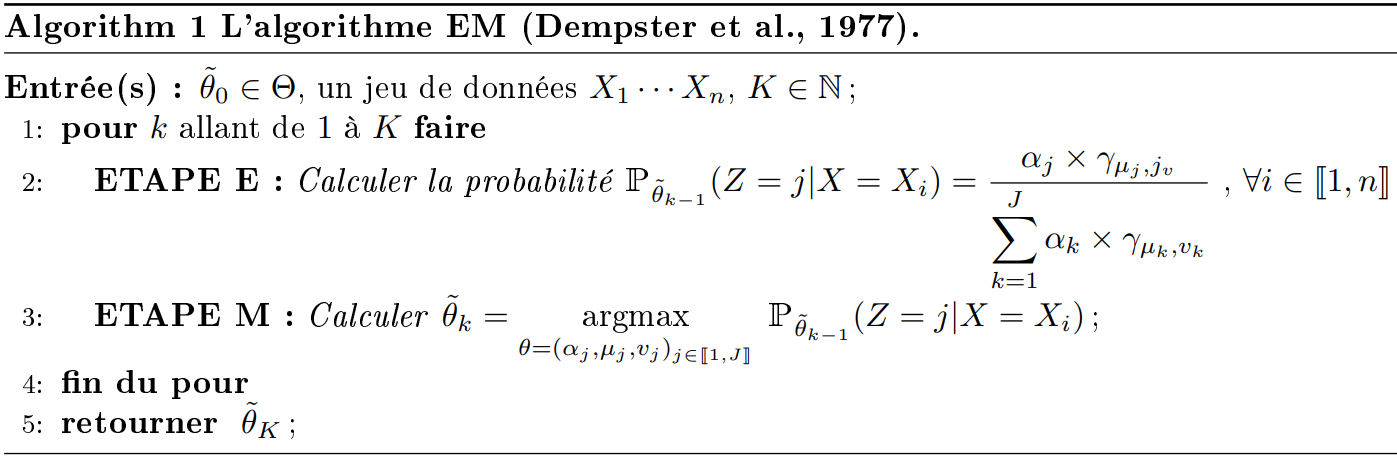
\includegraphics[scale=0.6]{images/pseudo_code.png}
		\end{figure}
	\end{frame}
	\begin{frame}{Les étapes de l'algorithme EM}
		\begin{block}{L'étape E (Expectation)}
			Consiste à déterminer $\mathbb{P}_{\tilde{\theta}}(Z = j | X = X_i)$ à l'aide de la formule suivante:
			\[
				\mathbb{P}_{\tilde{\theta}}(Z = j| X = X_i) = \frac{\alpha_j \times \gamma_{\mu_j, v_j}}{\sum_{k=1}^{J} \alpha_k \times \gamma_{\mu_k, v_k}}
			\]
		\end{block}
	\end{frame}
	\begin{frame}{Les étapes de l'algorithme EM}
		\begin{block}{L'étape M (Maximization)}
			Consiste à déterminer les EMV ($\widehat{\alpha_j}, \widehat{\mu_j}$, $\widehat{\sigma_j}$) de la log-vraisemblance conditionnelle via les formules suivantes:
			\begin{align*}
				\widehat{\alpha_j} &= \frac{1}{n}\sum_{i=1}^n \mathbb{P}_{\tilde{\theta}}(Z = j| X = X_i) \\
				\widehat{\mu_j} &= \frac{\sum_{i=1}^n X_i\mathbb{P}_{\tilde{\theta}}(Z = j| X = X_i)}{\sum_{i=1}^n \mathbb{P}_{\tilde{\theta}}(Z = j| X = X_i)} \\
				\widehat{v_j} &= \frac{\sum_{i=1}^n (X_i -\widehat{\mu_j})^2 \mathbb{P}_{\tilde{\theta}}(Z = j| X = X_i)}{\sum_{i=1}^n\mathbb{P}_{\tilde{\theta}}(Z = j| X = X_i)}
			\end{align*}
		\end{block}
	\end{frame}
	\section{Études de simulations}
	\begin{frame}{Cas des variables à "fortes séparations" }
		\begin{figure}[htp] 
			\centering
			\subfloat[Boxplot des erreurs pour $\alpha_1$, $\alpha_2$ et $\alpha_3$]{%
				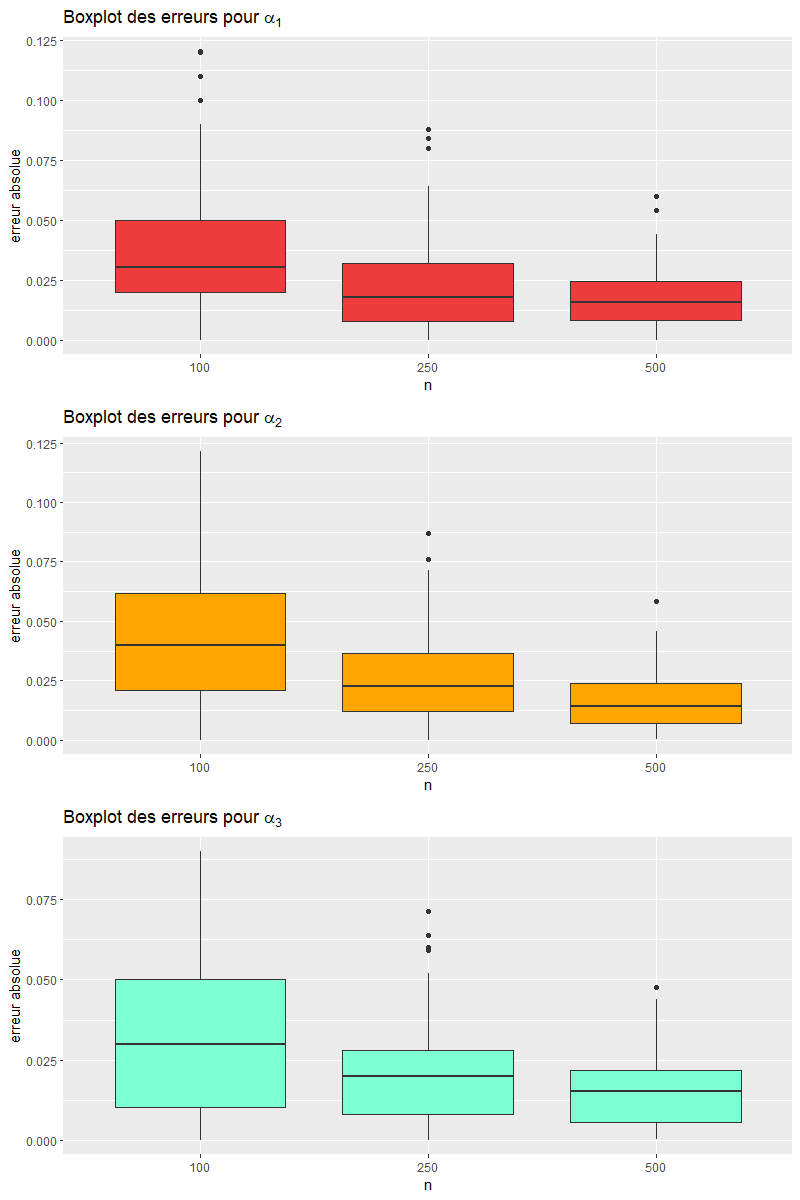
\includegraphics[scale=0.18]{images/good_alpha.png}%
			}%
			\hfill%
			\subfloat[Boxplot des erreurs pour $\mu_1$, $\mu_2$ et $\mu_3$]{%
				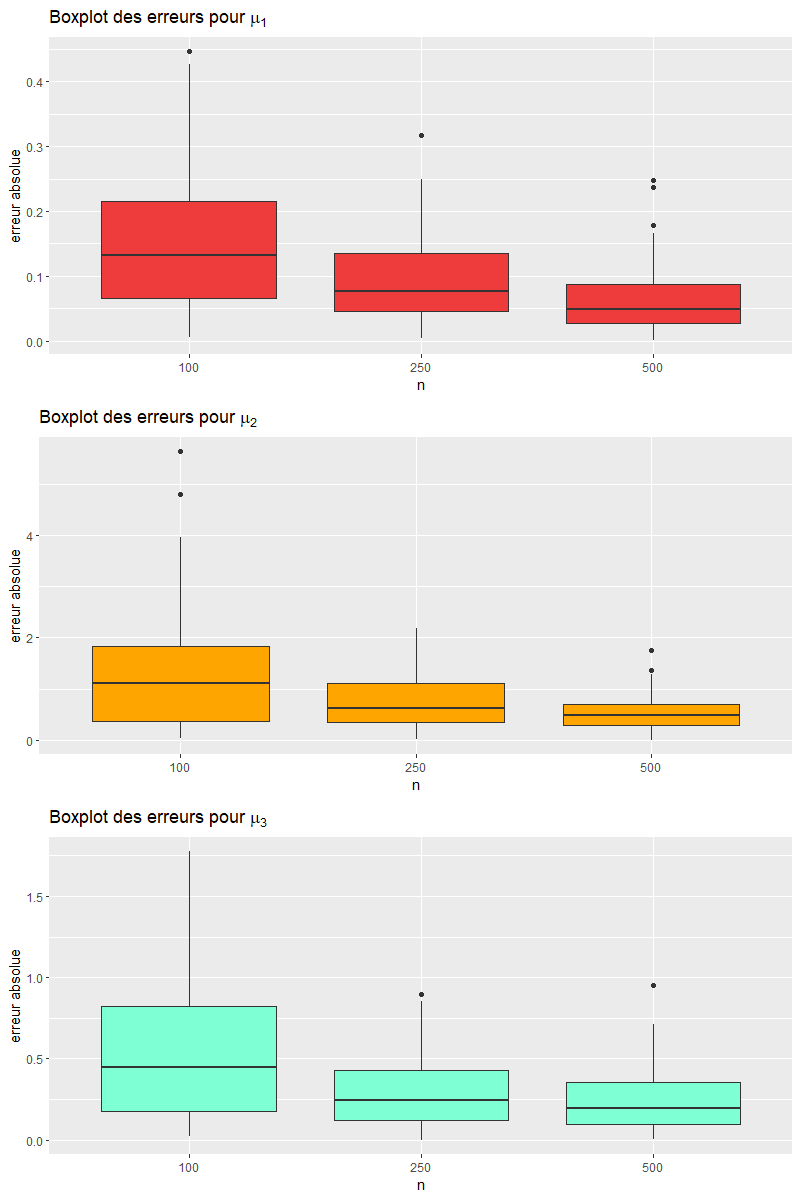
\includegraphics[scale=0.18]{images/good_mu.png}%
			}%
		\end{figure}
	\end{frame}

	\begin{frame}{Cas des variables à "faibles séparations" }
		\begin{figure}[htp] 
			\centering
			\subfloat[Boxplot des erreurs pour $\alpha_1$, $\alpha_2$ et $\alpha_3$]{%
				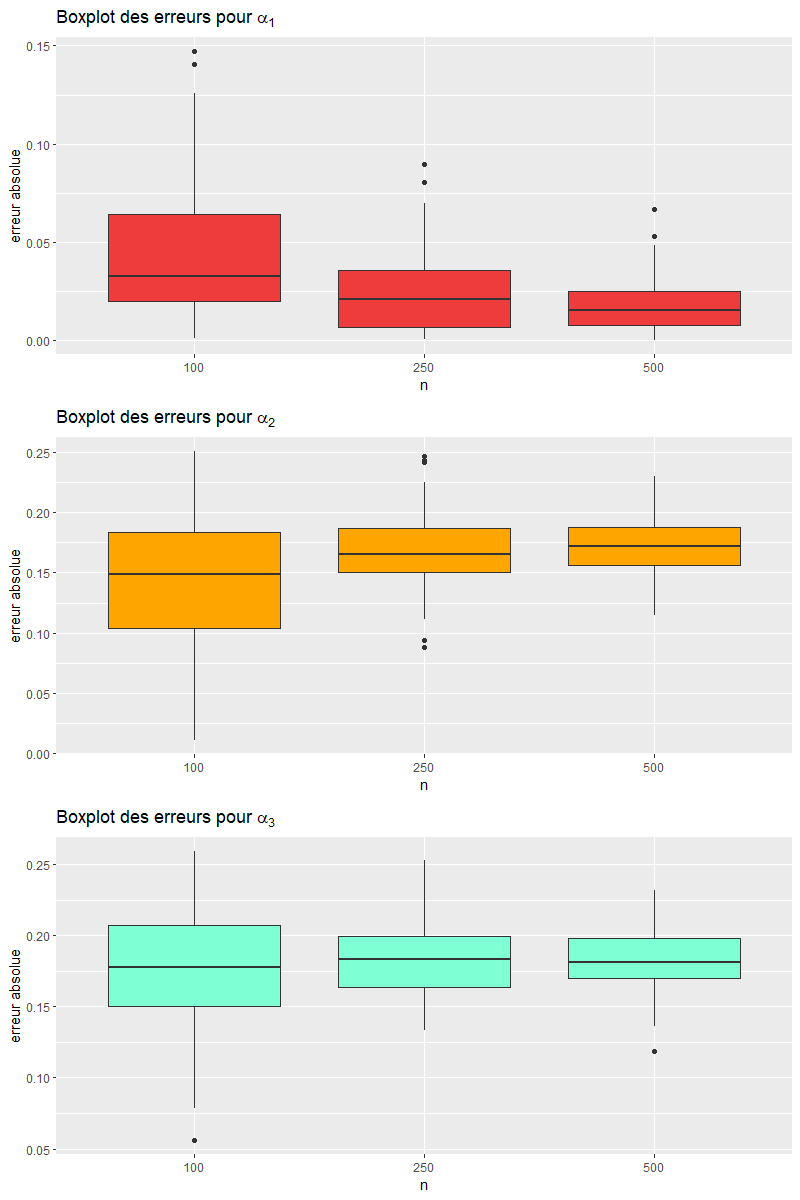
\includegraphics[scale=0.18]{images/bad_alpha.png}%
			}%
			\hfill%
			\subfloat[Boxplot des erreurs pour $\mu_1$, $\mu_2$ et $\mu_3$]{%
				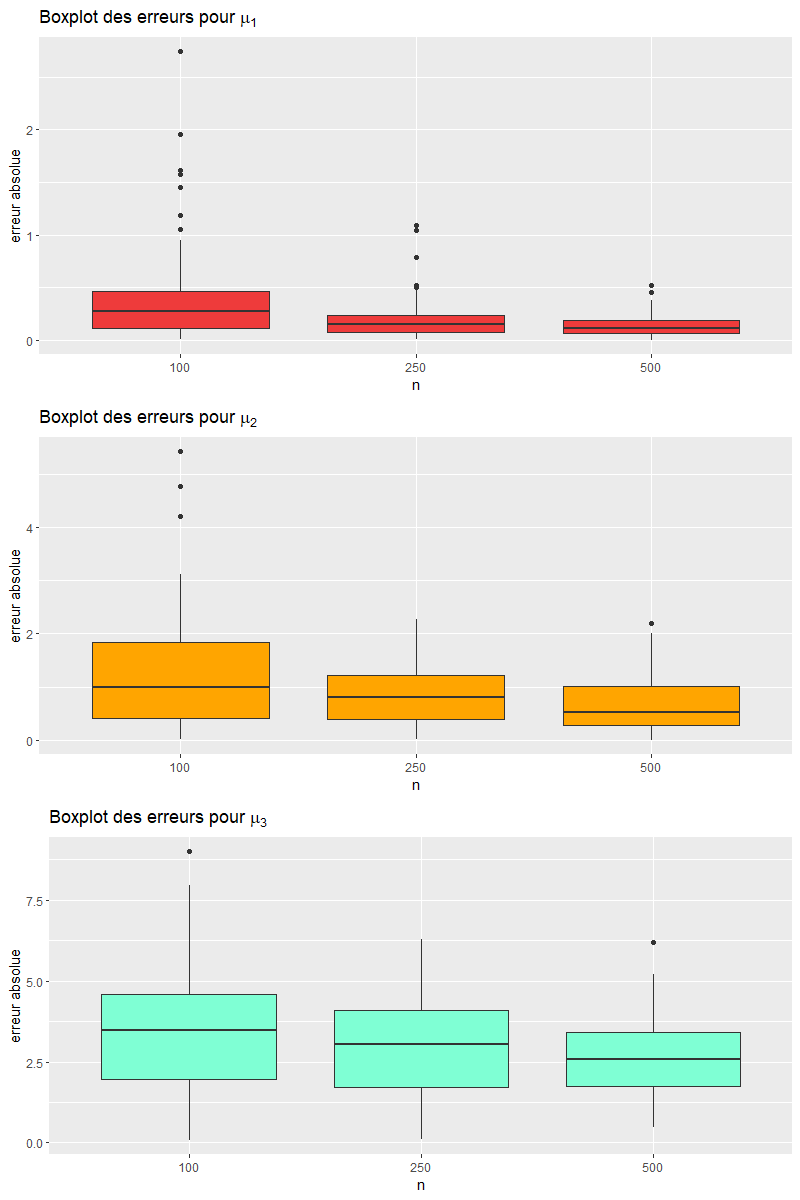
\includegraphics[scale=0.18]{images/bad_mu.png}%
			}%
		\end{figure}
	\end{frame}
	
	\section{Modélisation des nids d'oiseaux}
	
	\begin{frame}{Modélisation des nids d'oiseaux}
		\begin{block}{\scriptsize Première exploration des données}
			\begin{figure}[H]
				\centering
				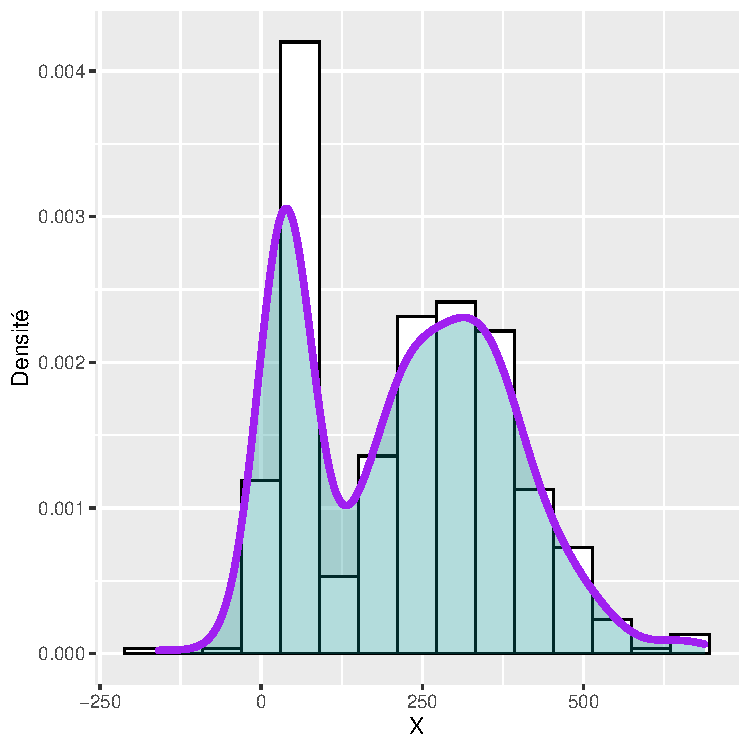
\includegraphics[scale=0.34]{dens1.pdf}
				\caption{Densité du mélange}
			\end{figure}
		\end{block}
	\end{frame}

	\begin{frame}{Heuristique graphique}
		\begin{block}{}
			\begin{figure}[H]
				\centering
				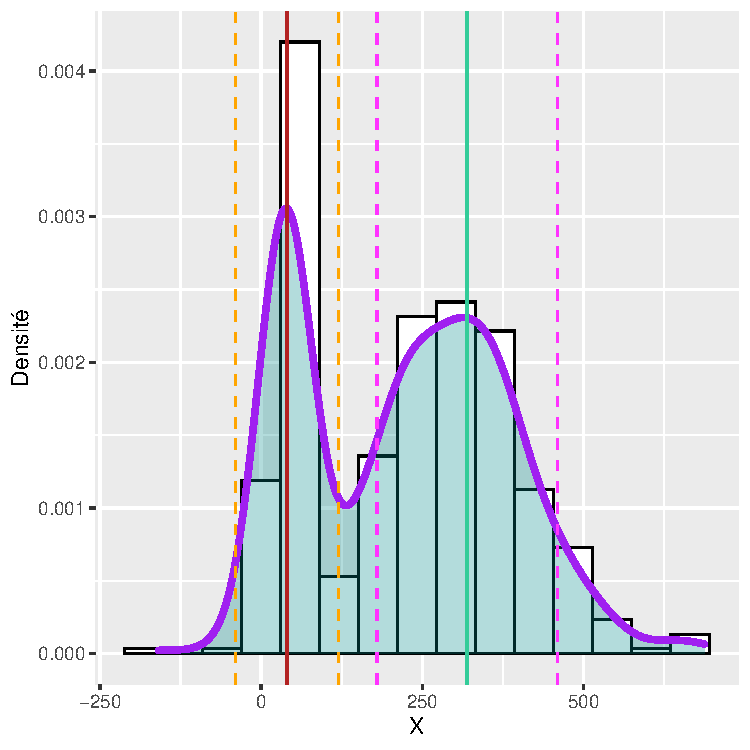
\includegraphics[scale=0.37]{dens1bis.pdf}
				\caption{Densité du mélange}
			\end{figure}
		\end{block}
	\end{frame}

	\section{Conclusion}

	\begin{frame}{Conclusion}
		\begin{block}{Conclusion}
			J'encule vos grosses marraines bien profond !!!
		\end{block}
	\end{frame}
\end{document}